\section{Диаграмма вариантов использования}
На рисунке \hyperref[use_case]{2.1} представленна Use Case диаграмма сценариев использования с описанными ранее видами акторов.


\begin{figure}[ph!] \label{use_case}
	\begin{center}
%		{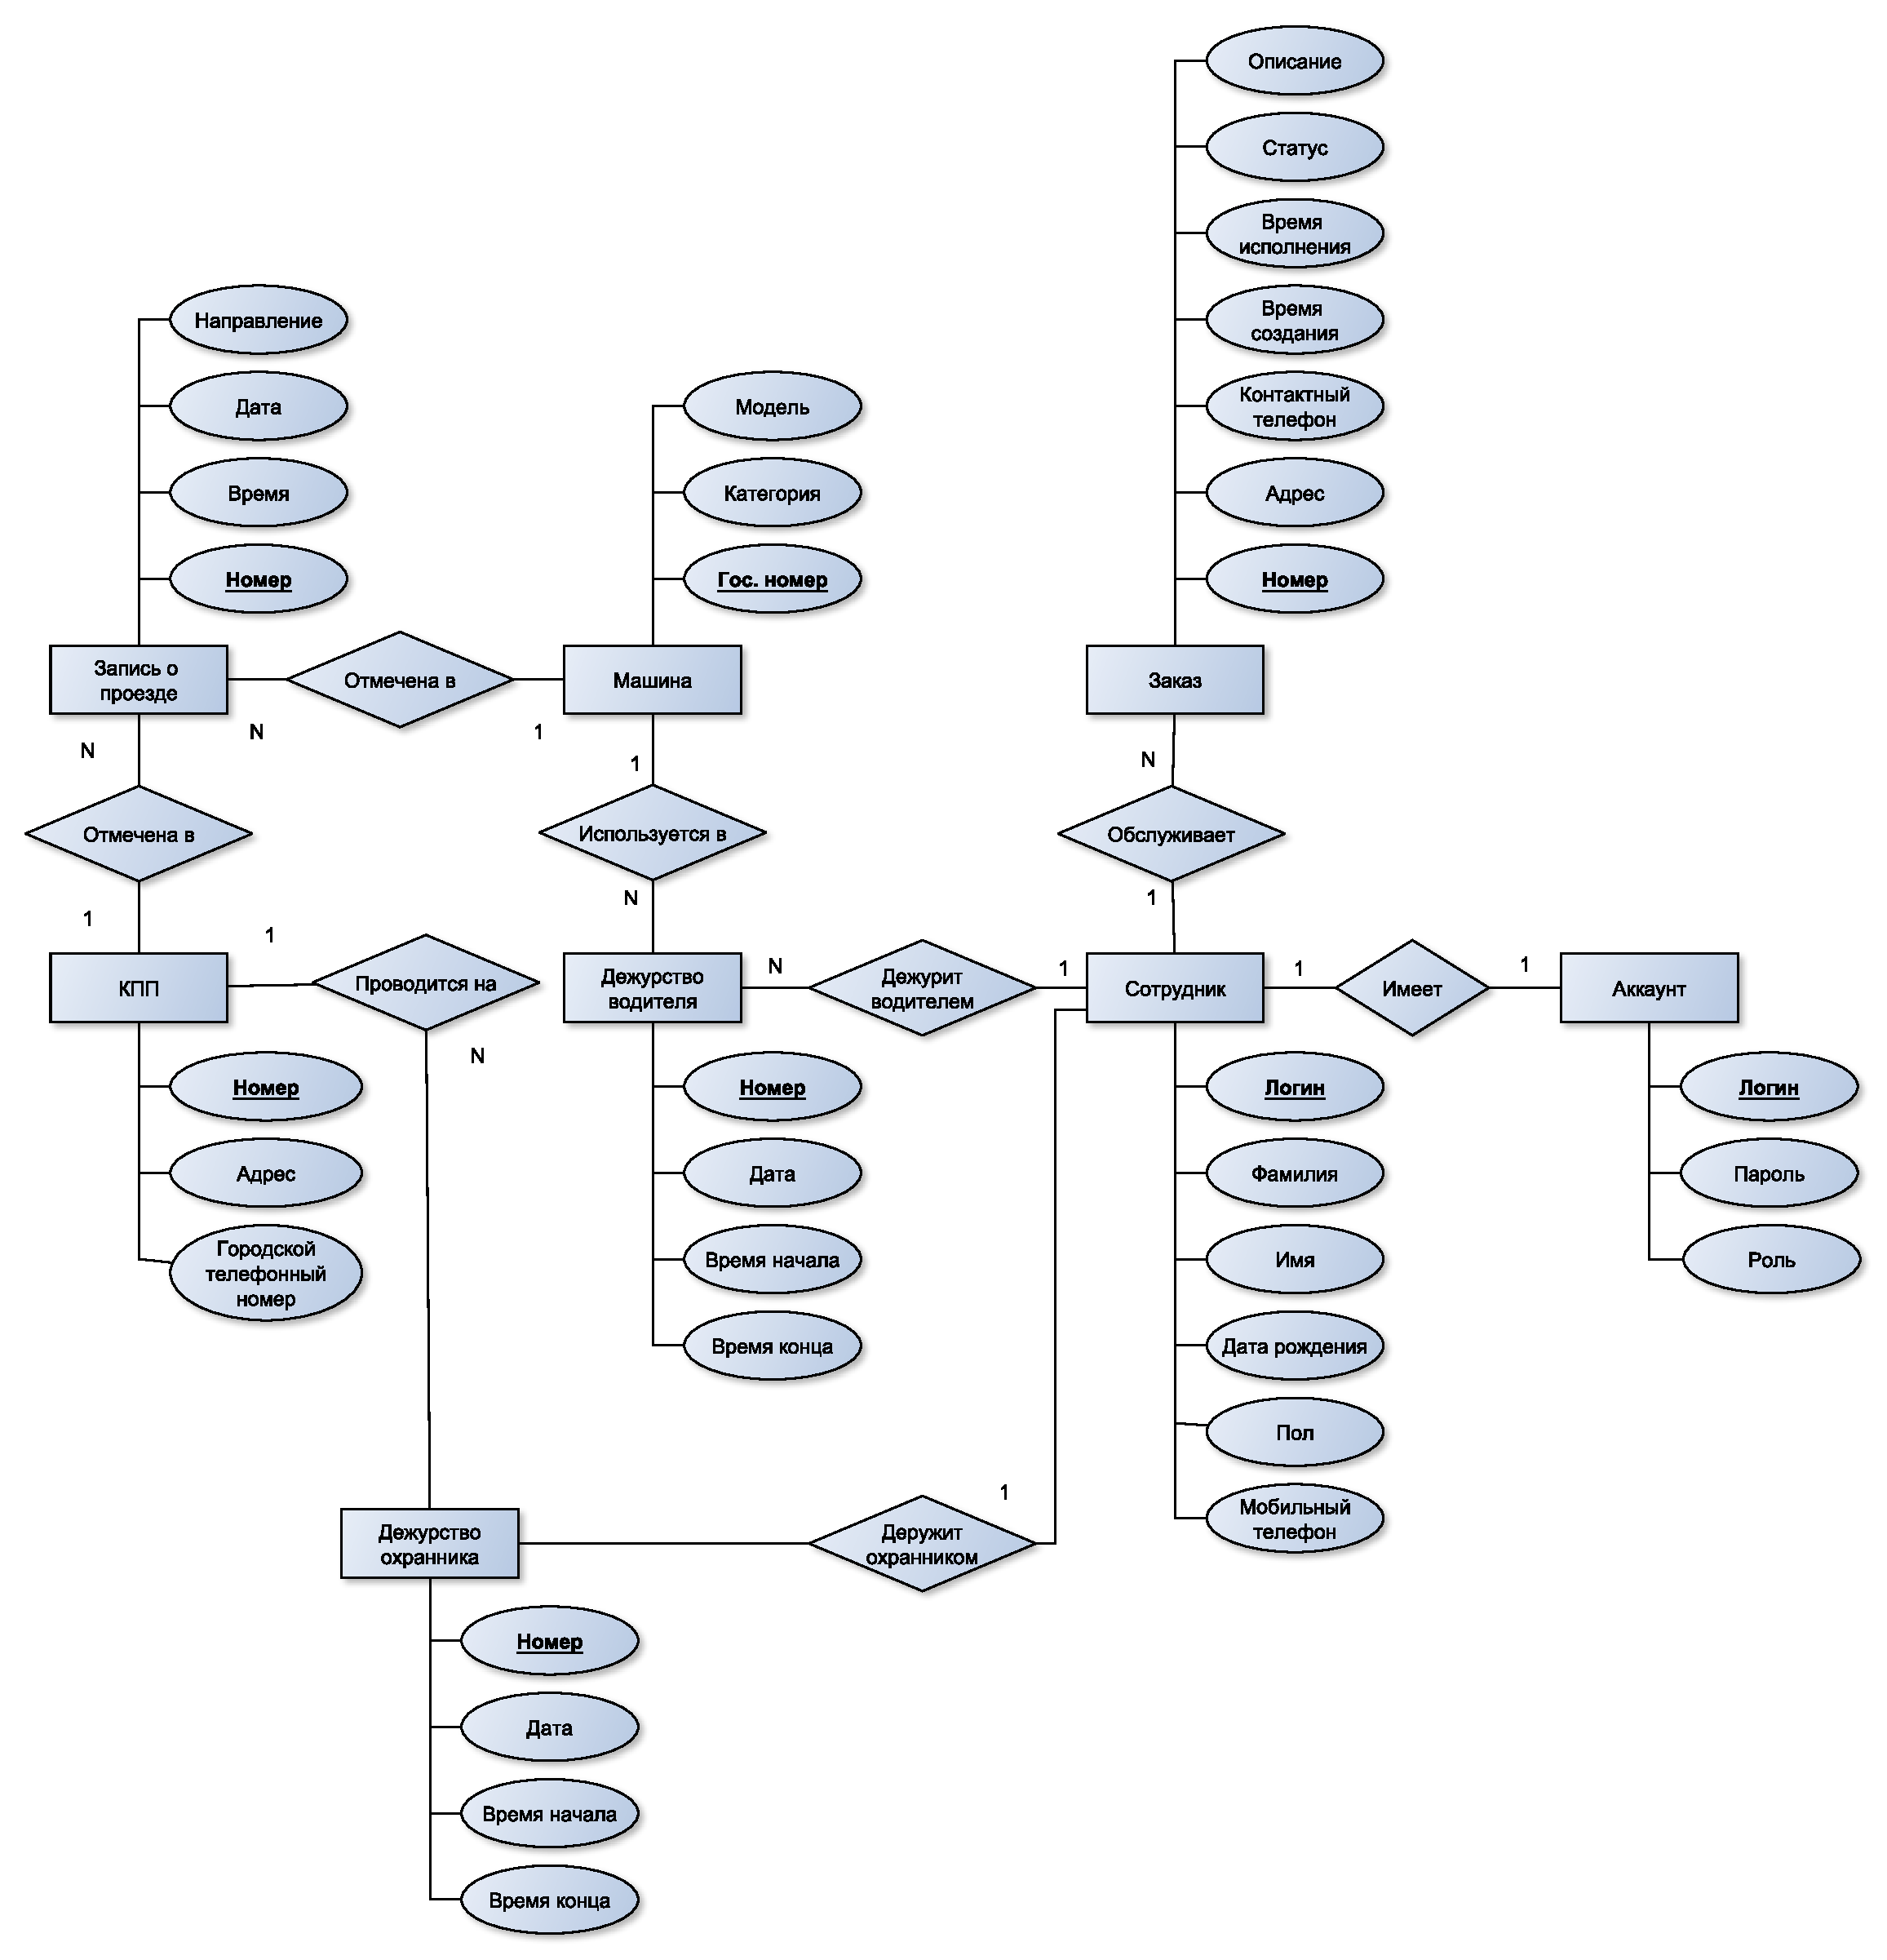
\includegraphics[height=18cm, width = 14cm]{schemes/er.pdf}}
		{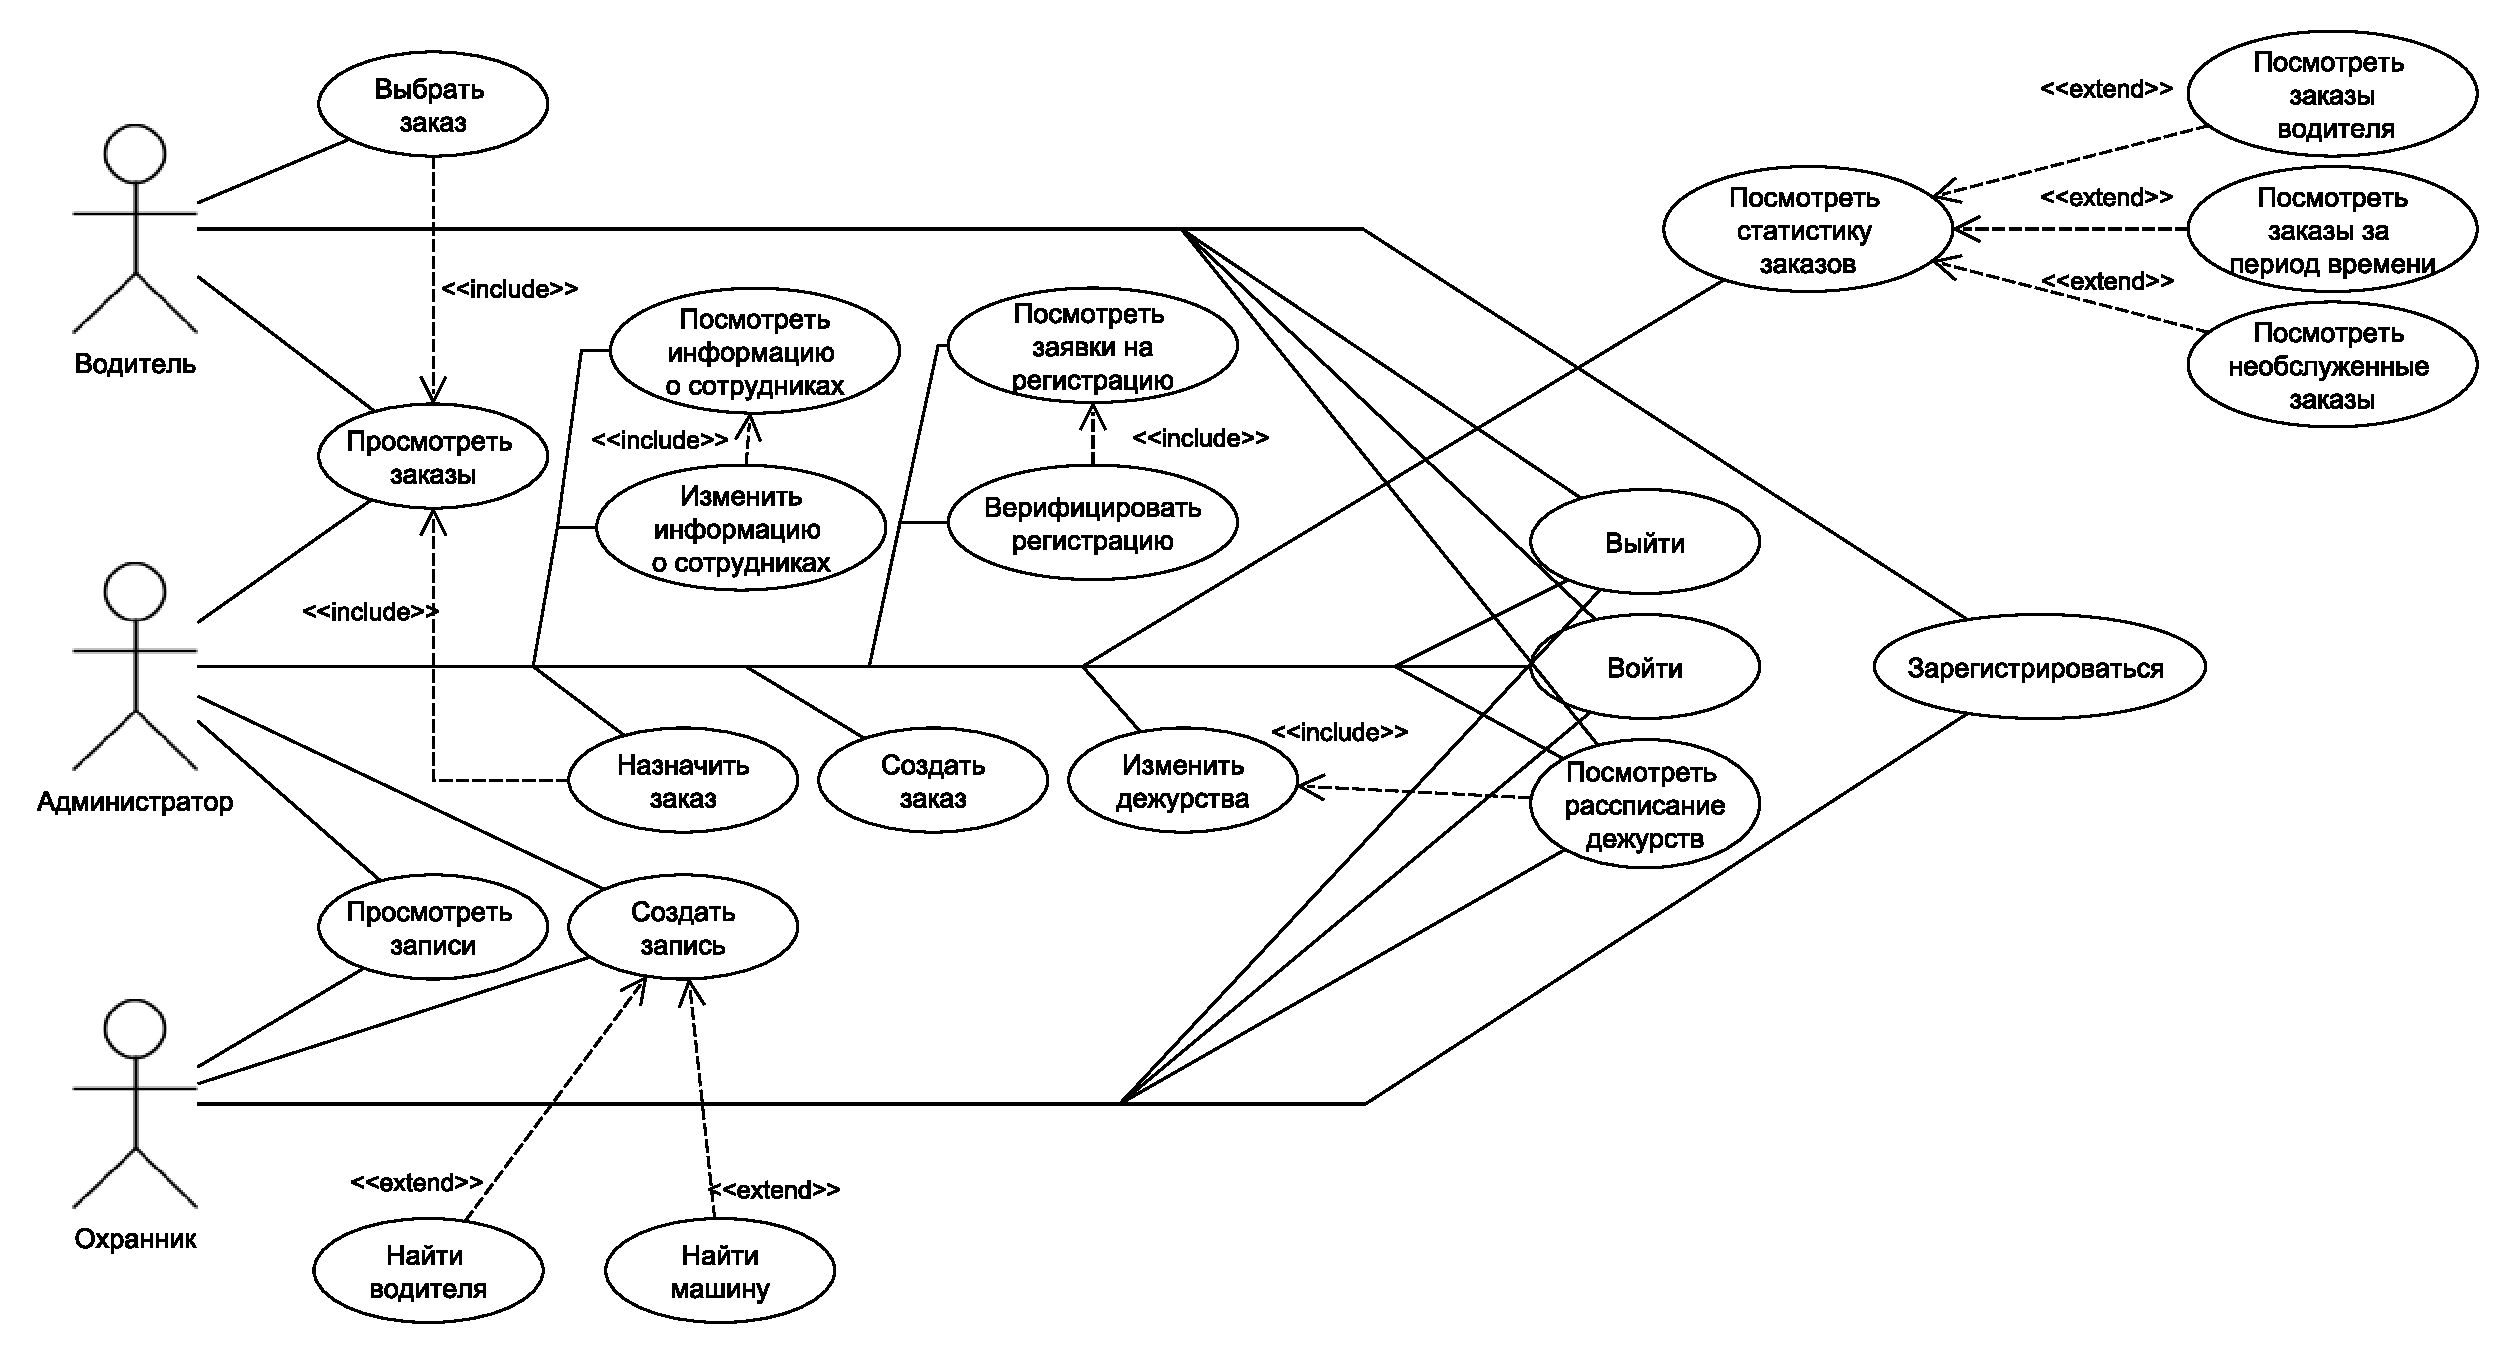
\includegraphics[scale=0.4, angle=-90]{schemes/use-case.pdf}}
		\caption{ER-диаграмма сущностей}
	\end{center}
\end{figure}


\section{Проектирование таблиц базы данных}
На рисунке \hyperref[er_db]{2.2} представленна ER-диаграмма сущностей базы данных.

\begin{figure}[ph!] \label{er_db}
	\begin{center}
		{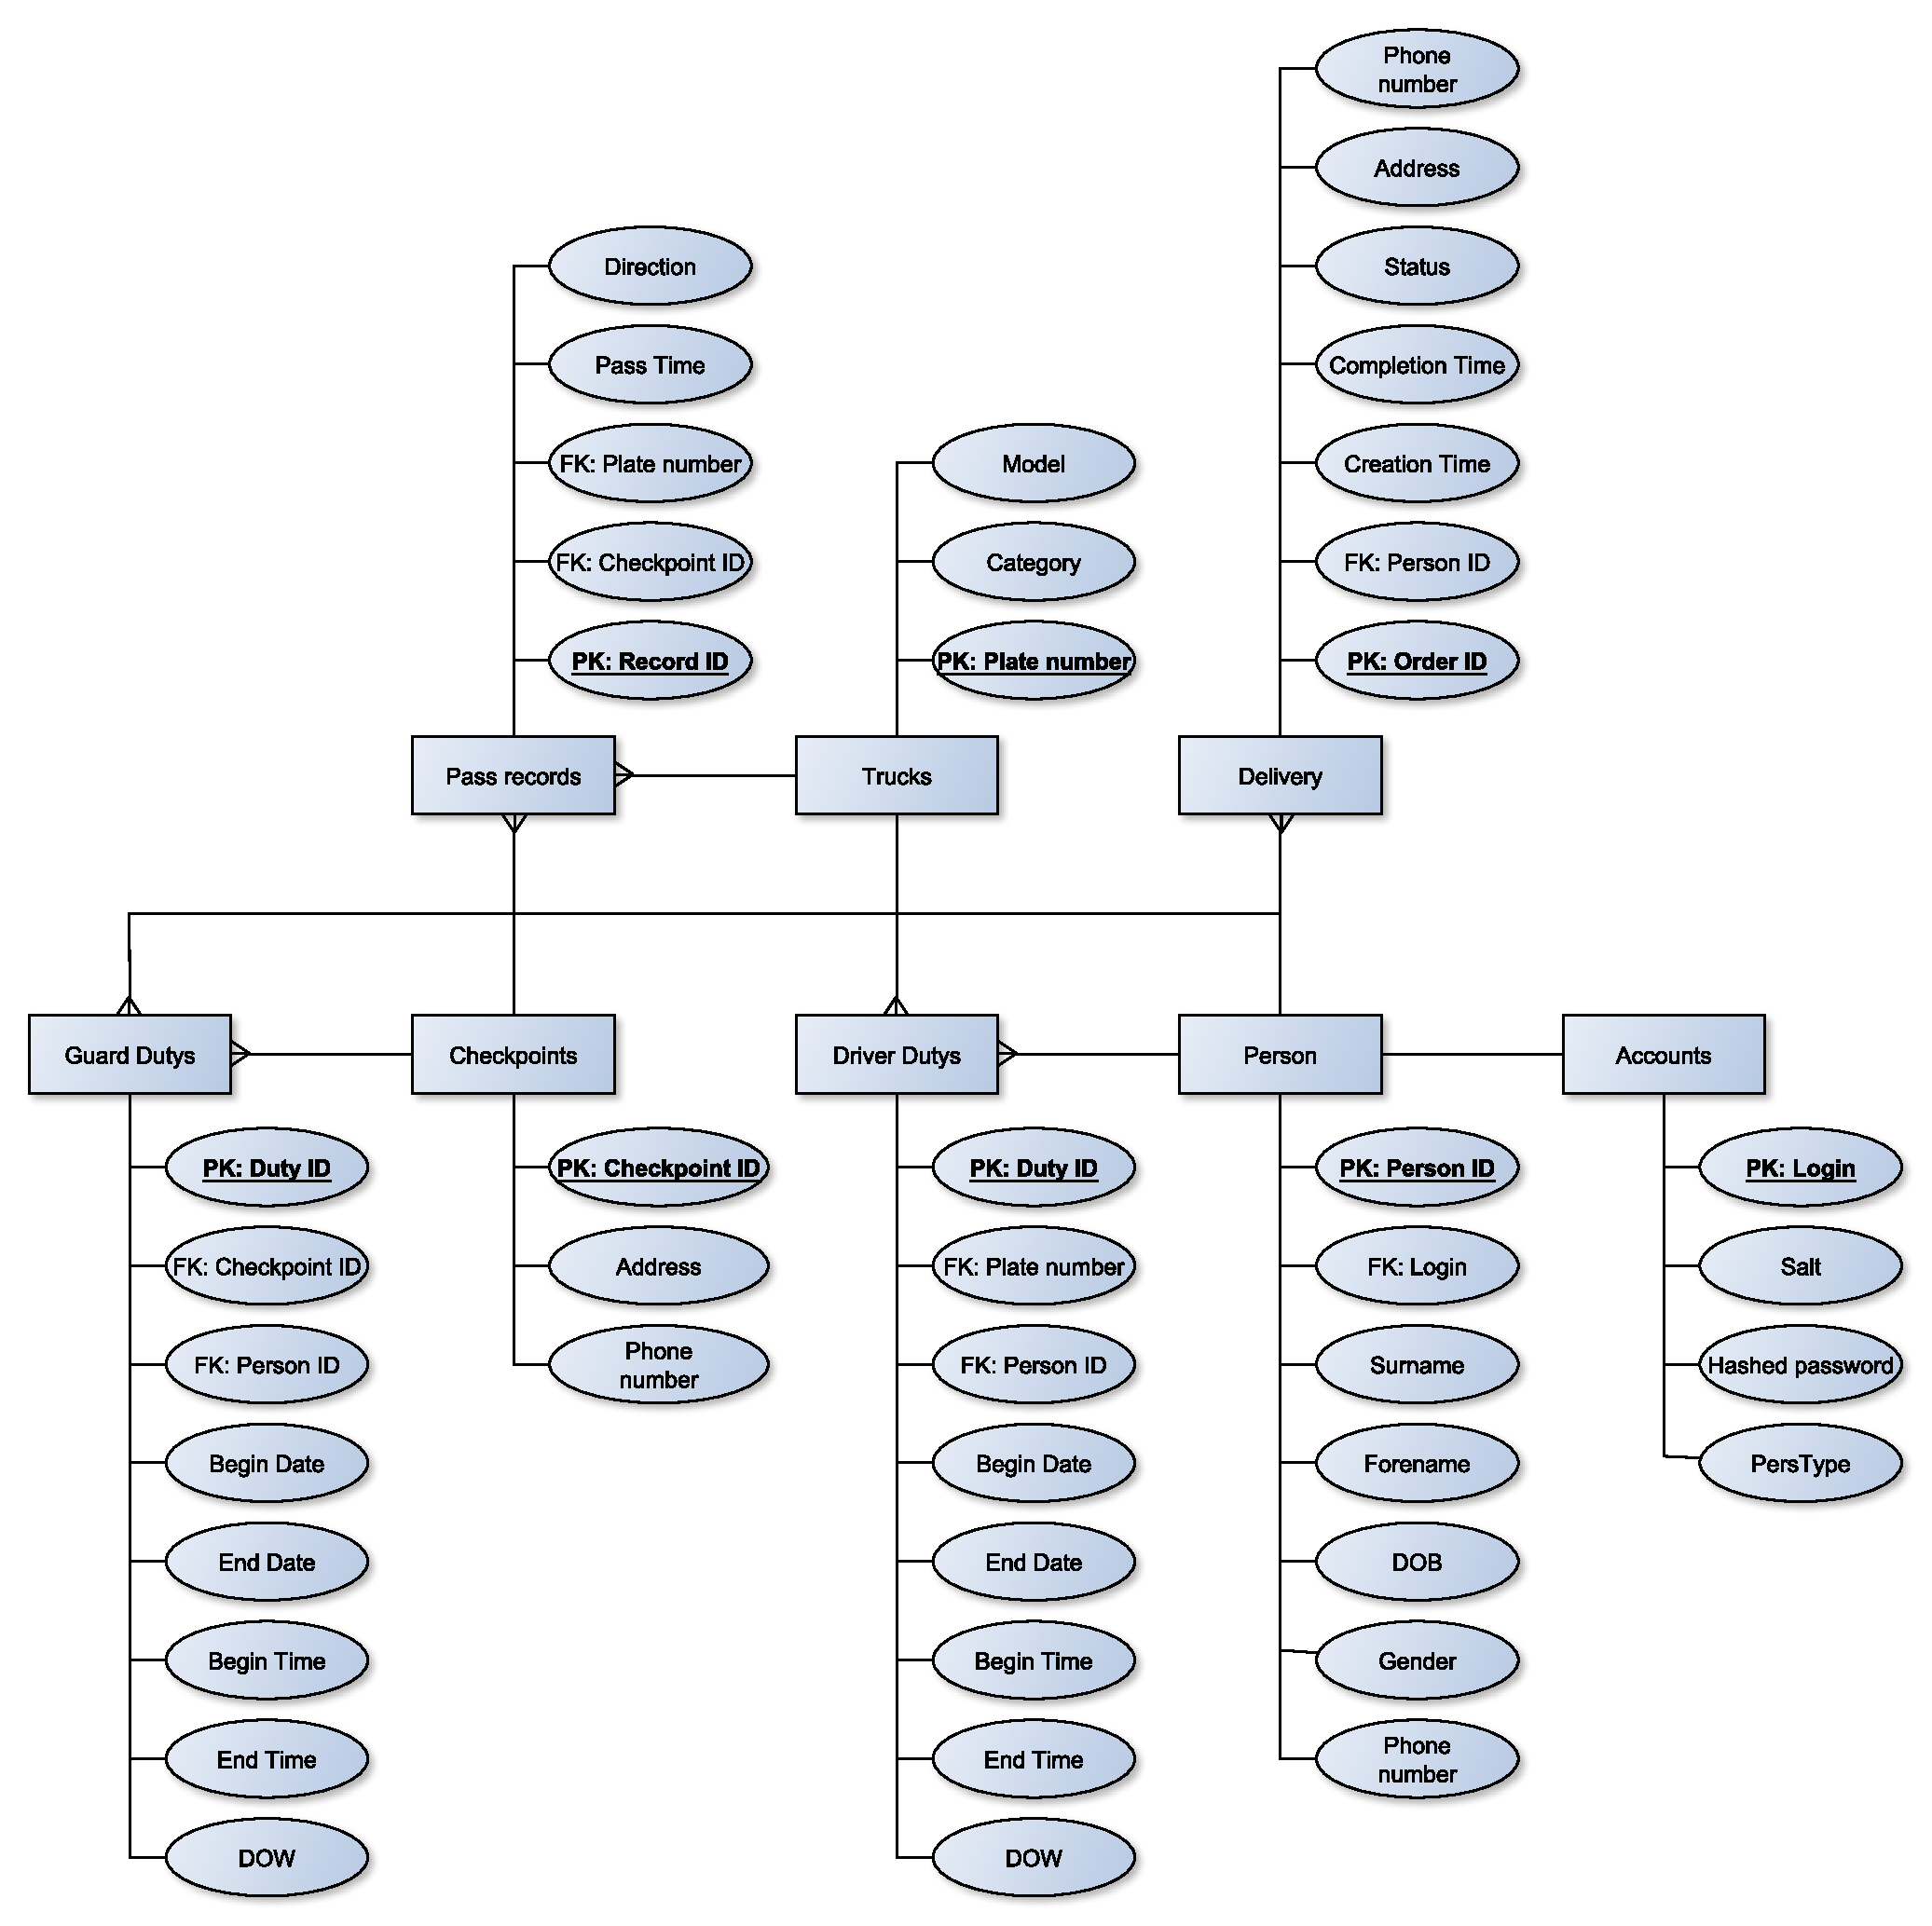
\includegraphics[height=14cm, width = 15cm]{schemes/er_db.pdf}}
%		{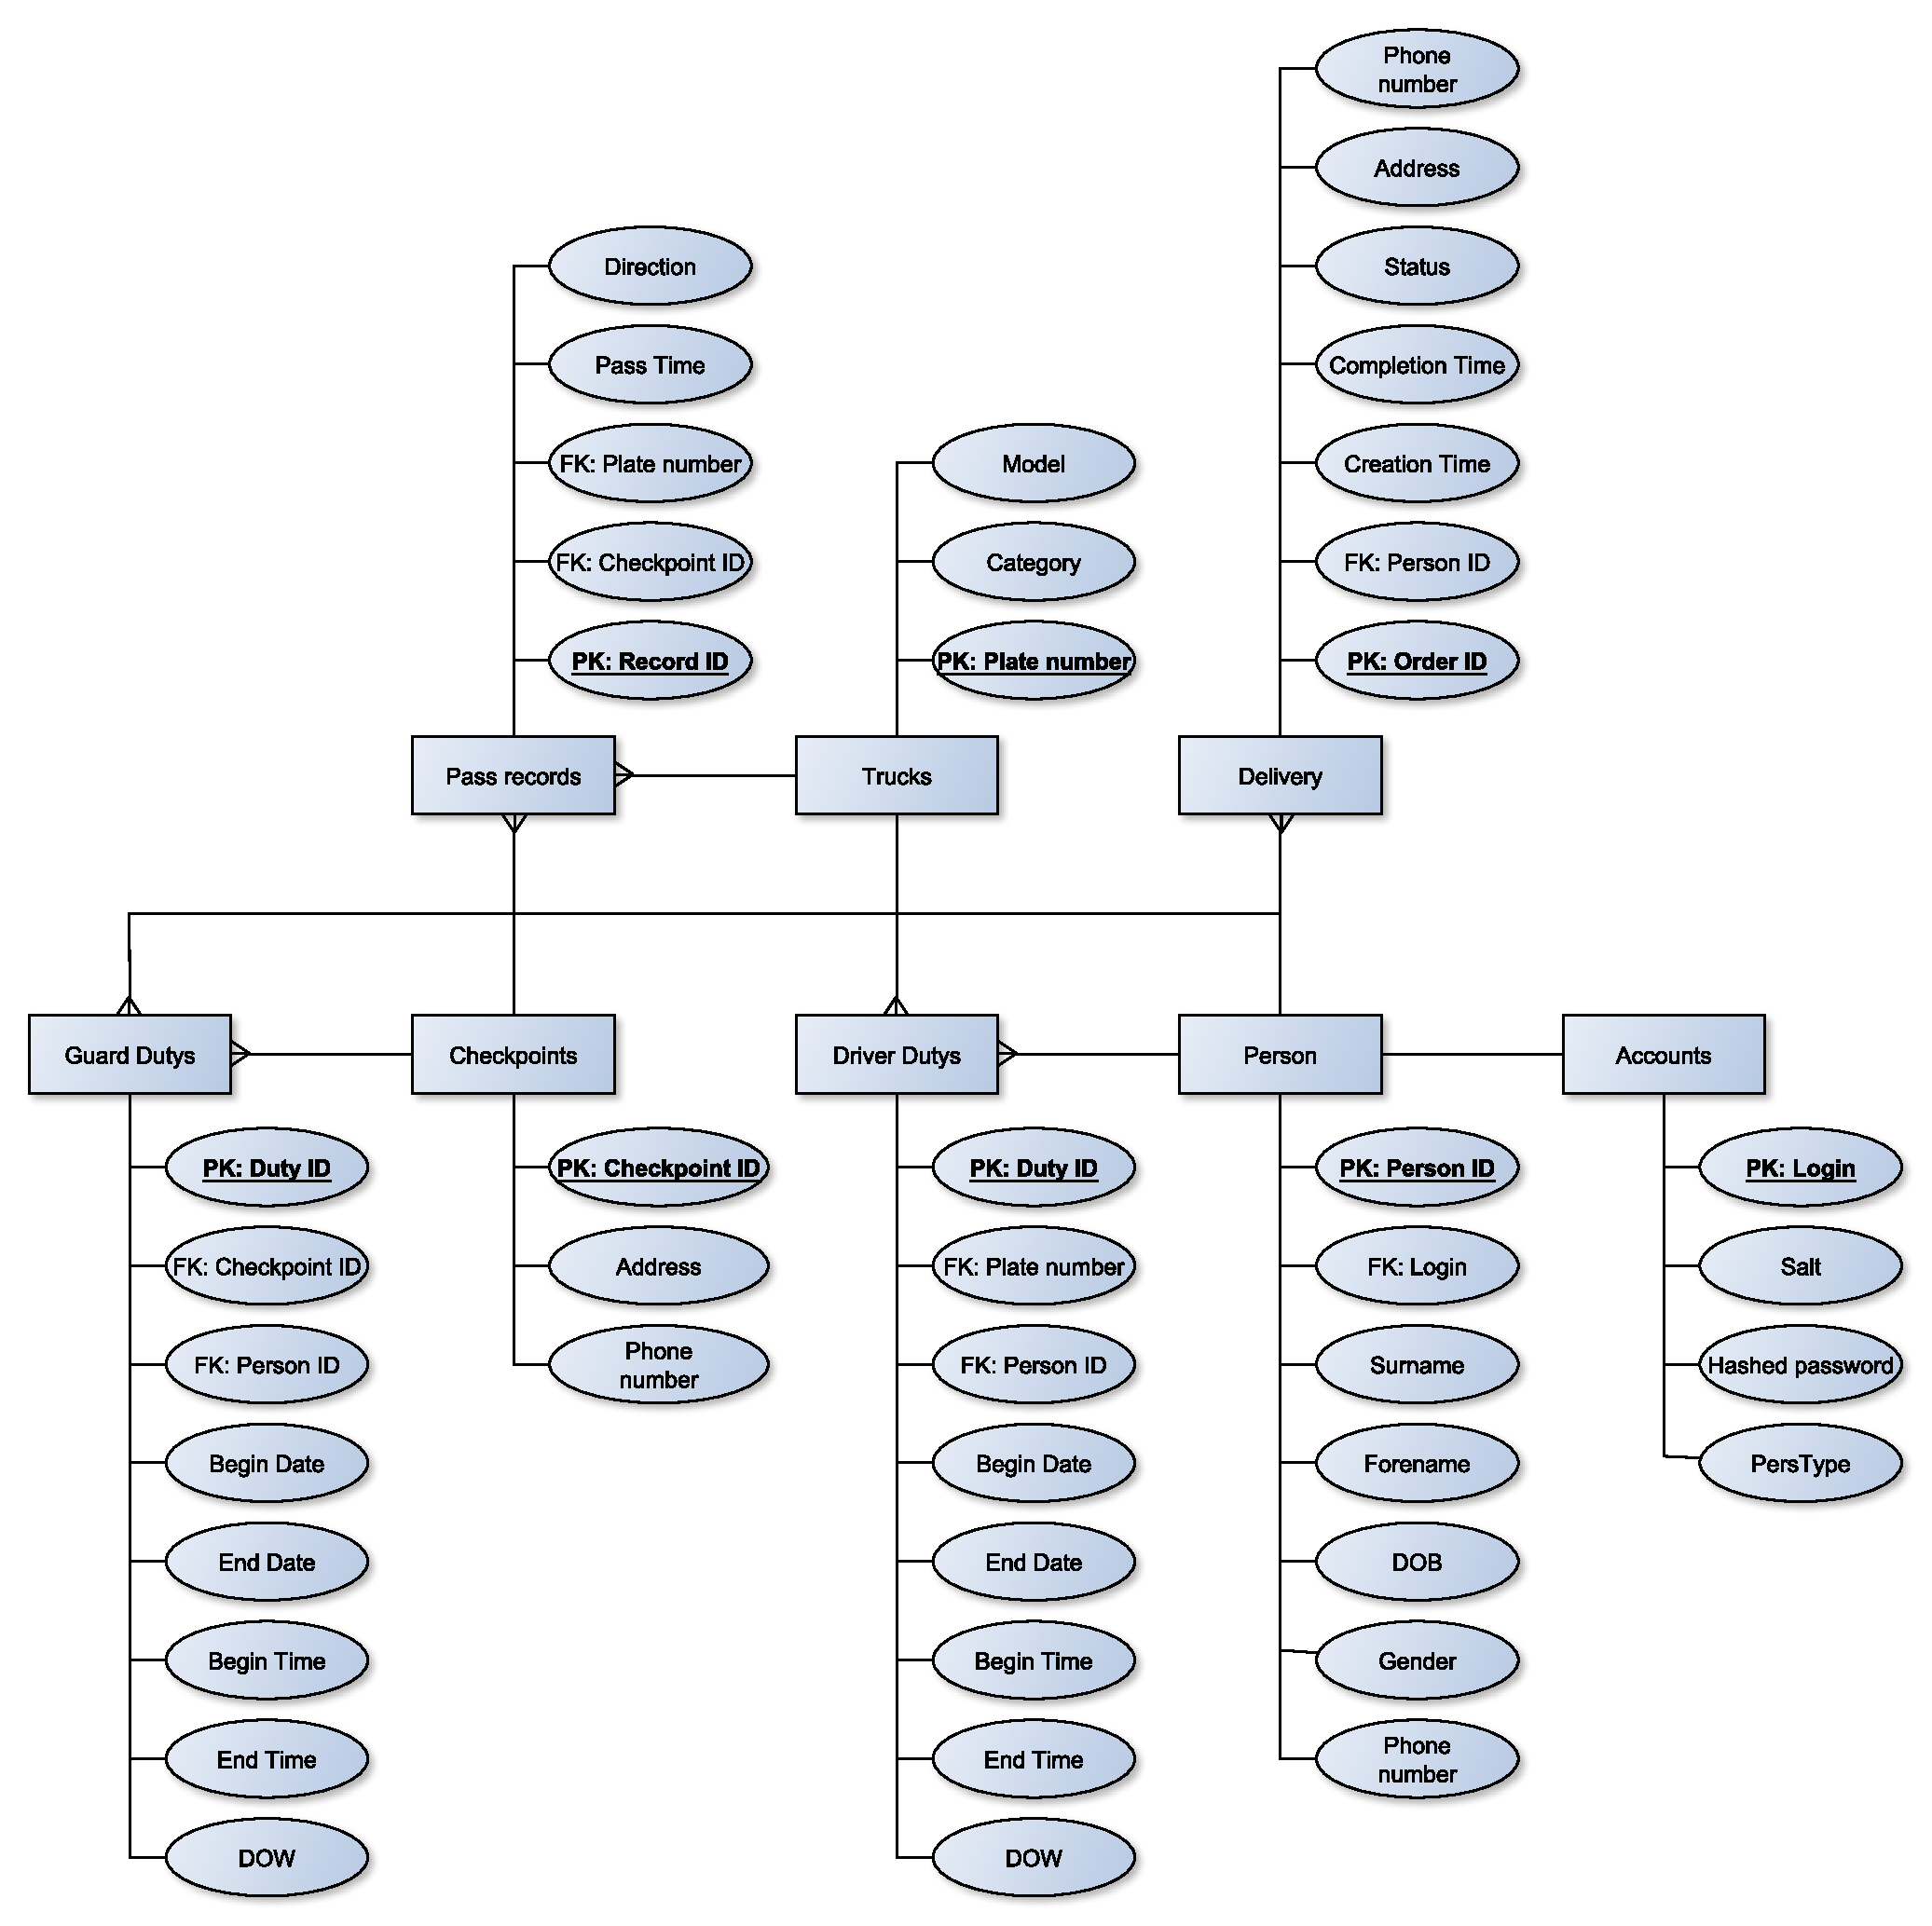
\includegraphics[scale=0.4, angle=0]{schemes/er_db.pdf}}
		\caption{ER-диаграмма сущностей базы данных}
	\end{center}
\end{figure}

На основании выделенных сущностей база данных должна содержать таблицы, описание которых приведено в таблицах 2.1-2.8

Для обеспечения приватности пароля к аккаунту было принято решение использовать хэширование. В качестве ролей используются значения admin, driver, guard (соотв. администратор, водитель, охранник).
\begin{table}[h] \label{acc_table}
	\begin{center}
	\caption{Accounts (таблица аккаунтов)}
	\begin{tabular}{| c | c | c |}
		\hline
		\textbf{Атрибут}		&	\textbf{Тип}		& \textbf{Комментарий} \\
		\hline
		Login 		&	Строка		&	Логин аккаунта, PK \\ \hline
		PersType 	&	Строка 		&	Роль аккаунта \\ \hline
		Salt 		&	Строка		&	"Соль" для хэширования пароля \\ \hline
		HashedPassword & Строка		&	Хэшированный пароль \\ \hline
	\end{tabular}
	\end{center}
\end{table}

\begin{table}[h] \label{pers_table}
	\begin{center}
		\caption{Person (таблица личной информации)}
		\begin{tabular}{| c | c | c |}
			\hline
			\textbf{Атрибут}		&	\textbf{Тип}		& \textbf{Комментарий} \\
			\hline
			Login 		&	Строка		&	Логин аккаунта, PK, FK \\ \hline
			Surname 	&	Строка 		&	Фамилия сотрудника \\ \hline
			Forename 	&	Строка 		&	Имя сотрудника \\ \hline
			DOB 		&	Дата		&	Дата рождения сотрудника \\ \hline
			Gender 		&   Строка		&	Пол сотрудника \\ \hline
			PhoneNumber	&   Строка		&	Номер мобильного телефона сотрудника \\ \hline
		\end{tabular}
	\end{center}
\end{table}

\begin{table}[h!] \label{truck_table}
	\begin{center}
		\caption{Trucks (таблица машин)}
		\begin{tabular}{| c | c | p{10cm} |}
			\hline
			\textbf{Атрибут}		&	\textbf{Тип}		& \textbf{Комментарий} \\
			\hline
			PlateNumber	&	Строка	&	Гос. номер машины, PK \\ \hline
			Category	&	Строка	&	Марка машины \\ \hline
			Model		&	Строка	&	Модель машины \\ \hline
		\end{tabular}
	\end{center}
\end{table}

В качестве статуса заказа используются значения not\_assigned, in\_transit, delivered (соотв. заказ не назначен водителю, заказ в процессе доставки и заказ доставлен).
\begin{table}[h!] \label{del_table}
	\begin{center}
		\caption{Delivery (таблица заказов)}
		\begin{tabular}{| c | c | p{10cm} |}
			\hline
			\textbf{Атрибут}		&	\textbf{Тип}		& \textbf{Комментарий} \\
			\hline
			OrderID		&	Целое число	&	Уникальный номер заказа, PK \\ \hline
			Login 		&	Строка		&	Логин водителя, доставляющего или доставившего заказ, FK \\ \hline
			Address 	&	Строка 		&	Адрес заказчика \\ \hline
			PhoneNumber	&	Строка 		&	Контакты заказчика \\ \hline
			Status 		& 	Строка		&	Статус заказа \\ \hline
			Description	& 	Строка		&	Содержание заказа \\ \hline
			CreationTime	& Дата, время	&	Дата и время создания заказа \\ \hline
			CompletionTime	& Дата, время	&	Дата и время завершения заказа \\ \hline
		\end{tabular}
	\end{center}
\end{table}

\begin{table}[h!] \label{checkp_table}
	\begin{center}
		\caption{Checkpoints (таблица КПП)}
		\begin{tabular}{| c | c | c |}
			\hline
			\textbf{Атрибут}		&	\textbf{Тип}		& \textbf{Комментарий} \\
			\hline
			CheckpointID	&	Целое число	&	Номер КПП, PK \\ \hline
			Address			&	Строка		&	Адрес КПП \\ \hline
			PhoneNumber		&	Строка		&	Номер телефона КПП \\ \hline
		\end{tabular}
	\end{center}
\end{table}


Дежурства как охранников, так и водителей имеют цикличный характер по неделе. Поэтому рациональнее хранить не каждое дежурство отдельно, а правило, содержащее диапазон дат и дни недели, в которые сотрудник дежурит. Атрибут дней недели в таблице хранит строку, определяющую дни по номеру (например строка 013 соответсвует дежурству по понедельникам, вторникам и четвергам). Период (или расписание) дежурства выделено в отдельную таблицу.

\begin{table}[h!] \label{dutyrule_table}
	\begin{center}
		\caption{DutyRules (таблица расписаний дежурств)}
		\begin{tabular}{| c | c | p{10cm} |}
			\hline
			\textbf{Атрибут}		&	\textbf{Тип}		& \textbf{Комментарий} \\
			\hline
			RuleID		&	Целое число	&	Номер периода дежурства, PK \\ \hline
			BeginDate 	&	Дата		&	Дата начала периода дежурства \\ \hline
			EndDate 	&	Дата		&	Дата окончания периода дежурства \\ \hline
			BeginTime 	&	Время		&	Время начала дежурства \\ \hline
			EndTime 	&	Время		&	Время окончания дежурства \\ \hline
			DOW 		&	Строка		&	Дни недели дежурства \\ \hline
		\end{tabular}
	\end{center}
\end{table}

\begin{table}[h!] \label{gduty_table}
	\begin{center}
		\caption{GuardDutys (таблица дежурств охранников)}
		\begin{tabular}{| c | c | p{10cm} |}
			\hline
			\textbf{Атрибут}		&	\textbf{Тип}		& \textbf{Комментарий} \\
			\hline
			DutyID		&	Целое число	&	Номер дежурства, PK \\ \hline
			Login 		&	Строка		&	Логин дежурящего охранника, FK \\ \hline
			CheckpointID &	Целое число	&	Номер КПП, FK \\ \hline
			RuleID		&	Целое число	&	Номер периода дежурства, FK \\ \hline
		\end{tabular}
	\end{center}
\end{table}

\begin{table}[h!] \label{dduty_table}
	\begin{center}
		\caption{DriverDutys (таблица дежурств водителей)}
		\begin{tabular}{| c | c | p{10cm} |}
			\hline
			\textbf{Атрибут}		&	\textbf{Тип}		& \textbf{Комментарий} \\
			\hline
			DutyID		&	Целое число	&	Номер дежурства, PK \\ \hline
			Login 		&	Строка		&	Логин дежурящего водителя, FK \\ \hline
			PlateNumber &	Строка		&	Гос. номер машины, FK \\ \hline
			RuleID		&	Целое число	&	Номер периода дежурства, FK \\ \hline
		\end{tabular}
	\end{center}
\end{table}

В качестве направления проезда используются значения in, out (соотв. въезд и выезд с территории предприятия).
\newpage
\begin{table}[h!] \label{pass_table}
	\begin{center}
		\caption{PassRecords (таблица записей проездов)}
		\begin{tabular}{| c | c | c |}
			\hline
			\textbf{Атрибут}		&	\textbf{Тип}		& \textbf{Комментарий} \\
			\hline
			RecordID	&	Целое число	&	Номер записи, PK \\ \hline
			PlateNumber	&	Строка		&	Гос. номер машины, FK \\ \hline
			CheckpointID &	Целое число	&	Номер КПП, FK \\ \hline
			PassTime 	&	Дата, время	&	Дата и время проезда \\ \hline
			Direction 	&	Строка		&	Направление проезда \\ \hline
		\end{tabular}
	\end{center}
\end{table}

\section{Архитектура приложения}
Наиболее известным подходом к проектированию архитектуры web-приложения является шаблон MVC. Данный паттерн предполагает разделение приложения на три описанные части.
\begin{itemize}
	\item Model (модель) - компонент бизнес-логики, отвечает за взаимодействие с базой данной и основную обработку информации.
	\item View (представление) - компонент, отвечающий за отображения данных, полученных в результате работы модели.
	\item Controller (контроллер) - компонент, отвечающий за получение запроса от пользователя, передачу их модели для дальнейшего обновления представления;
\end{itemize}

В данной курсовой работе будет использован описанный подход, так как он чётко разграничивает зоны каждого компонента, что позволяет сделать их независимыми.


\section*{Вывод}
Результатом конструкторской части стала разработка сценариев использования приложения, его архитектуры и проектирование таблиц базы данных.



